\paragraph{QuizziPedia::Front-End::ModelViews::TopicKeywordsModelView}
				
				\label{QuizziPedia::Front-End::ModelViews::TopicKeywordsModelView}
				
				\begin{figure}[ht]
					\centering
					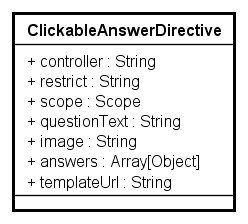
\includegraphics[scale=0.5,keepaspectratio]{UML/Classi/Front-End/QuizziPedia_Front-end_Templates_ClickableAnswerTemplate.png}
					\caption{QuizziPedia::Front-End::ModelViews::TopicKeywordsModelView}
				\end{figure} \FloatBarrier
				
				\begin{itemize}
					\item \textbf{Descrizione}: classe di tipo modelview la cui istanziazione è contenuta all'interno della variabile di ambiente \$scope di \textit{Angular.js\ped{G}}. All'interno di essa sono presenti le variabili e i metodi necessari per il \textit{Two-Way Data-Binding\ped{G}} tra la view \texttt{CreateQuestionnaireView} e il controller \texttt{KeywordsController};
					\item \textbf{Utilizzo}: viene utilizzata per effettuare il \textit{Two-Way Data-Binding\ped{G}} tra la view \texttt{CreateQuestionnaireView} e il controller \texttt{KeywordsController} rendendo disponibili variabili e metodi;
					\item \textbf{Relazioni con altre classi}: 
					\begin{itemize}
						\item \textit{IN} \texttt{CreateQuestionnaireView}: view per la creazione del questionario; 
						\item \textit{IN} \texttt{TopicKeywordsController}: questa classe permette di gestire il recupero delle parole chiave di un questionario;
					\end{itemize}
					\item \textbf{Attributi}: 
					\begin{itemize}
						\item \texttt{+ topics: Array} \\ Array contenente le stringhe dei nomi degli argomenti;
						\item \texttt{+ keyword: String} \\ Attributo contenente la keyword associata alla domanda/questionario;
					\end{itemize}
					\item \textbf{Metodi}: 
					\begin{itemize}
						\item \texttt{+} \texttt{getKeywords(key: String): String[]}: \\ Metodo che ritorna le parole che hanno a che fare con key
						
						\textbf{Parametri}:
						\begin{itemize}
							\item \texttt{key: String}: parametro che identifica la stringa con la quale cercare le keywords. 
						\end{itemize}
					\end{itemize}
				\end{itemize}
				
					